\section{Zielsetzung}
In diesem Versuch soll mittels zweier Scan-Verfahren ein Acrylblock mit Bohrungen vermessen werden (A-Scan und B-Scan).
Wird das Herzschlagvolumen eines Modellherzes gemessen.

\section{Theorie}
Als Ultraschall wird Schall mit einer Frequenz von \SI{20}{\kilo \hertz} bis \SI{1}{\giga \hertz}
beschrieben. Diese Schallfrequenzen kommen in der Medizin in Diagnostik und Therapie zum Einsatz.
Schall ist eine longitudinale Welle, die in einem Medium mittels Druckschwankungen weitergeleitet
wird:
\FloatBarrier
\begin{align*}
  p(x,t) = p_0 + v_0~Z \symup{cos}(\omega t - kx)
\end{align*}
\FloatBarrier
In dieser Gleichung beschreibt $Z$ die akustische Impedanz, welche durch die Dichte $\rho$ und die
Schallgeschwindigkeit $c$ im vorliegenden Stoff beschrieben wird:
\FloatBarrier
\begin{align*}
  Z = c \cdot \rho
\end{align*}
\FloatBarrier
Bei Schallwellen ist die Phasengeschwindigkeit auf Grund von Dichte und Druckschwankungen materialabhängig.
Sie zeigen also im Gegensatz zu elektromagnetischen Wellen Dispersion. Alle anderen grundlegenden
Eigenschaften der elektromagnetischen Wellen zeigen Schallwellen ebenso.
Im Versuch ist lediglich die Schallweiterleitung in Festkörpern von Bedeutung, welche durch
folgenden Zusammenhang zwischen $E$, dem Elastizitätsmodul und der Dichte $\rho$ beschrieben wird:
\FloatBarrier
\begin{align*}
  c_{\symup{\tiny{FK}}} = \sqrt{\frac{E}{\rho}}
\end{align*}
\FloatBarrier
Hierbei ist zu beachten, dass $c_{\symup{\tiny{FK}}}$ für transversale und longitudinale Wellen
unterschiedlich aussieht.
Breiten sich Schallwellen in einem Festkörper aus, so verlieren diese durch Absorption exponentiell an Energie.
Somit wird die Intensität einer Welle durch folgenden Zusammenhang beschrieben:
\FloatBarrier
\begin{align*}
  I(x) = I_0 \cdot \symup{e}^{(-\alpha ~ x)}
\end{align*}
\FloatBarrier
In dieser Gleichung beschreibt $\alpha$ den Absorptionskoeffizienten, $I_0$ die Anfangsintensität und $x$
die zurückgelegte Strecke.
Der Absorptionskoeffizient ist für Luft sehr groß, weshalb im Versuch darauf zu achten ist, dass
stets ein Kontaktmittel zwischen Ultraschallkopf und zu untersuchendem Körper verwendet wird.
Bei dem Kontaktmittel handelt es sich um Hydrogel oder bidestilliertes Wasser.
Treffen Schallwellen auf Grenzflächen, so werden sie reflektiert. Die Reflexion kann durch den
Reflexionskoeffizienten $R$ beschrieben werden, für dessen Berechnung die Impedanzen der beiden
Materialien, die die Grenzfläche bilden, wichtig sind:
\FloatBarrier
\begin{align*}
  R = \left(\frac{Z_1 - Z_2}{Z_1 + Z_2} \right)^2
\end{align*}
\FloatBarrier
Der Reflexionskoeffizient gibt das Verhältnis zwischen einlaufender und reflektierter Welle an.
Folglich ergibt sich der Transmissionskoeffizient zu $T = 1 ~ - R$.
Um Ultraschallwellen zu erzeugen, wird der Piezoelektrische Effekt verwendet, wobei ein piezoelektrischer
Kristall (Quarz) mittels eines elektrischen Feldes in Schwingung versetzt wird, wodurch dieser
Ultraschallwellen emittiert. Das elektrische Feld übt eine Kraft auf die einzelnen Ladungen im Kristallgitter aus,
welches sich daraufhin zusammenzieht oder ausdehnt und somit beginnt zu schwingen. Umgekehrt können Schallwellen
das Kristallgitter in Schwingung versetzen, wodurch sich der Ladungsschwerpunkt verschiebt und folglich eine
Spannung anliegt. So kann der piezoelektrische Effekt ebenso zur Detektion von Ultarschallwellen genutzt werden.
Mittels Ultraschall ist es so möglich Aussagen über die Beschaffenheit von Körpern zu treffen, ohne diese eröffnen
zu müssen.
Dies kann auf zwei verschiedene Arten geschehen. Zum einen, indem von einem Sender ein kurzer Schallimpuls durch das
Medium ausgesendet wird, welcher von einem Detektor auf der anderen Seite des zu utersuchenden Körpers aufgefangen wird.
Mögliche Fehlstellen sind durch eine Abschwächung des Signals zu erkennen. Die Lokalisation dieser ist jedoch nicht möglich.
Dieses Verfahren wird Durchschallungsverfahren genannt und ist schematisch in Abbildung \ref{abb1} zu sehen.
\FloatBarrier
\begin{figure}
  \centering
  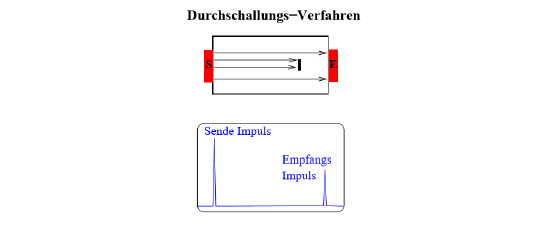
\includegraphics[scale=0.8]{1.PNG}
  \caption{Schematische Darstellung des Durchschallungsverfahrens.\cite{Q1}}
  \label{abb1}
\end{figure}
\FloatBarrier
Das zweite Verfahren, das bei der Unteruschung von Medien zum Einsatz kommt, ist das Impuls-Echo-Verfahren.
Hierbei fungiert der Schallkopf sowohl als Sender als auch als Empfänger, der an den Grenzflächen
emittierten Ultraschallwellen. Wie aus Abbildung \ref{abb2} hervorgeht, ist es mittels dieser Methode möglich,
etwaige Fehlstellen zu detektieren. Deren Größe kann durch die Höhe der gemessenen Reflexion abgeschätzt werden.
Ist die Schallgeschwindigkeit im Medium bekannt, so kann mittels folgender Formel ebenfalls die Lage der
Fehlstelle ermittelt werden:
\FloatBarrier
\begin{align*}
  s = \frac{1}{2} c ~ t
\end{align*}

\FloatBarrier
\begin{figure}
  \centering
  
\includegraphics[scale=0.7]{2.PNG}
  \caption{Schematische Darstellung des Impuls-Echo-Verfahrens. \cite{Q1}}
  \label{abb2}
\end{figure}
\FloatBarrier


\section{Durchführung}
Bevor mit den Scans begonnen wird, muss der Acrylblock mittels einer Schieblehre ausgemessen werden. Der Acrylblock ist schematisch in Abbildung
\ref{abb3} zu sehen.
\begin{figure}
  \centering
  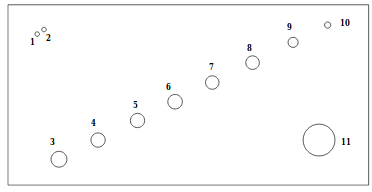
\includegraphics[scale=0.5]{Acrylbox.png}
  \caption{Schematische Ansicht des Acylblockes. \cite{Q1}}
  \label{abb3}
\end{figure}
Im ersten Versuchsteil soll dieser Acrylblock nun mit Hilfe eines A-Scans vermessen werden. Hierzu wird eine \SI{1}{\mega\hertz}-Sonde mit Wasser
auf der Oberseite des Blocks gekoppelt. Um den Abstand der Löcher von der Oberseite des Acrylblocks zu ermitteln, wird die Sonde direkt über das zu
vermessenen Loch gesetzt und ein A-Scan durchgeführt, bei dem die Spannung $U$ gegen die Zeit $t$ aufgetragen wird.
Es wird die Zeit des reflektierten Impulses von dem entstehenden Graphen abgelesen.
Dieses wird für jede einzelne Bohrung durchgeführt. Bei der doppelten Bohrung muss gegebenenfalls der zeitlich spätere Bereich verstärkt werden, um
die Peaks genau abmessen zu können.
Nachdem alle Bohrungen vermessen sind, wird der Block gedreht und das selbe von der anderen Seite durchgeführt.

Im zweiten Teil des Versuchs sollen die Bohrungen 1 und 2 (siehe \ref{abb3}) genauer untersucht werden, da diese durch den ersten Versuchsteil kaum
zu differenzieren sind. Hierzu sollen Bilder eines A-Scans von den Bohrungen 1 und 2 gemacht werden. Zunächst wird ein A-Scan mit einer
\SI{1}{\mega\hertz}-Sonde durchgeführt, wie im vorherigen Versuchsteil. Danach wird eine \SI{2}{\mega\hertz}-Sonde angeschlossen und erneut ein
A-Scan durchgeführt, um beide Bohrungen besser unterscheiden zu können. Auch hier werden die reflektieren Signale für größere Zeiten verstärkt,
um die Peaks besser ablesen zu können.

Der selbe Acrylblock soll im dritten Versuchsteil durch einen B-Scan vermessen werden. Hierzu wird erneut eine \SI{1}{\mega\hertz}-Sonde auf der
Oberseite des Acrylblocks mit Wasser als Verbindungsschicht gekoppelt. Nun wird bei dem Programm auf B-Scan umgestellt und gestartet. Während das
Programm läuft, wird die Sonde langsam über die Oberfläche des Acrylblocks geschoben. Das enstehende Diagramm wird gespeichert.
Auch bei diesem Versuchsteil wird der Block gedreht und es wird erneut ein B-Scan von der Unterseite des Acrylblock durchgeführt.

Im letzten Versuchsteil soll das Herzzeitvolumen eines Herzmodells gemessen werden. Hierzu wird das Herzmodell zu einem Drittel mit
destilliertem Wasser befüllt und eine \SI{1}{\mega\hertz}-Sonde darüber angebracht, sodass diese so eben das Wasser berührt.
Nun wird ein A-Scan durchgeführt und die Zeit des reflektierten Schalls gemessen. Daraufhin wird das Herzmodell mittels eines Gummiballs
aufgepumpt und in diesem Zustand erneut ein A-Scan durchgeführt und die Zeit des reflektierten Schalls gemessen.
Nun wird ein B-Scan des Herzmodells durchgeführt, indem das Herzmodell mittels des Gummiballs periodisch aufgepumpt wird. Dabei
sollten mindestens 5 Herzschläge simuliert werden. Die Frequenz sollte hierbei möglichst konstant bleiben. Zuletzt wird
der Durchmesser des Herzmodells mittels einer Schieblehre bestimmt.

\section{Auswertung}
\subsection{Lage und Breite der Störstellen}
Im ersten Teil des Versuchs wird die Höhe und Breite der Störstellen im Acrylblock zum einen mittels eines
A-Scans und zum anderen mittels eines B-Scans ermittelt.
Die Messwerte zur Ermittlung der Lage der Störstelle mittels des A-Scans sind in Tabelle \ref{tab1} zu finden.
Die berechneten Ergebnisse sind zusammen mit den Ergebnissen, die mit der Schieblehre ermittelt wurden in Tabelle \ref{tab2} zu finden.
Hierbei sind $d_b$, $s_b$ und $l_b$ die berechneten Werte und $d_m$, $s_m$ und $l_m$ die mit der Schieblehre gemessenen Werte.
Es ist bei der Berechnung der Werte $d$ und $s$ zu beachten, dass hier das Impuls-Echo-Verfahren angewendet wurde, weshalb die
Laufzeit zwischen den beiden Peaks $\Delta t$ durch zwei dividiert werden muss, wenn die Lage der Störstellen
bestimmt wird. Die Strecken $d_{\symup{i}}$ und $s_{\symup{i}}$ werden somit mit Hilfe folgeneder Formel berechnet:
\FloatBarrier
\begin{align}
  \label{eq1}
  d_{\symup{i}} / s_{\symup{i}} = v_{\symup{Acryl}} \cdot \frac{\Delta t}{2}
\end{align}
\FloatBarrier
Hierbei ist $v_{\symup{Acryl}}$ die Schallgeschwindigkeit in Acryl, die $\SI{2730}{\metre \per \second}$ beträgt \cite{Q2}
und $d$ der Abstand der Oberkante des Blocks bis zur Störstelle und $s$ der Abstand der Unterkante des Blocks zur
Störstelle, wenn der Block wie in Abbildung \ref{abb1} auf dem Tisch steht. Die Nummerierung der Störstellen erfolgt ebenfalls
wie in Abbildung \ref{abb3} zu sehen. Die Dicke der Störstelle $l$ ergibt sich folglich aus der Differenz der, zuvor
mit der Schieblehre bestimmten, Höhe des Acrylblocks $h$ = $\SI{8,25(5)}{\cm}$ und den beiden Größen $s$ und $d$:
\FloatBarrier
\begin{align}
  \label{eq2}
  l = h -(s + d)
\end{align}
\FloatBarrier


\noindent Da die Schieblehre einen Fehler von $\SI{0,05}{\cm}$ bestitzt, ist zu beachten, dass bei allen Werten, die mit Hilfe abgemessener Werte berechnet
werden dieser Fehler für jeden abgemessenen Wert hinzuaddiert werden muss.
\FloatBarrier
\begin{table}
  \centering
  \caption{Messwerte zur Ermittlung der Lage der Störstellen im Acrylblock.}
  \label{tab1}
  \begin{tabular}{c c c c c c c }
    \toprule
      Störstelle & $t_1$ / $\si{\micro \second}$ & $t_2$ / $\si{\micro \second}$ & $\Delta t_d$ / $\si{\micro \second}$ &  $t_3$ / $\si{\micro \second}$ & $t_4$ / $\si{\micro \second}$ & $\Delta t_s$ / $\si{\micro \second}$ \\
              \midrule
              3  &  2,22  &  46,77  &  44,55   &  2,12  &  11,43  &  9,31    \\
              4  &  2,12  &  41,37  &  39,25   &  2,12  &  17,67  & 15,55    \\
              5  &  2,12  &  35,66  &  33,54   &  2,12  &  24,02  & 21,90    \\
              6  &  2,01  &  30,16  &  28,15   &  2,12  &  30,05  & 27,93    \\
              7  &  2,01  &  24,44  &  22,43   &  2,12  &  36,19  & 34,07    \\
              8  &  2,12  &  18,52  &  16,40   &  2,12  &  42,01  & 39,89    \\
              9  &  2,12  &  12,70  &  10,58   &  2,12  &  47,83  & 45,71    \\
              10 &  2,12  &   6,77  &   4,65   &  2,12  &  -      & -        \\
              11 &  2,12  &  42,43  &  40,31   &  2,12  &  12,85  & 10,73    \\
              \bottomrule
            \end{tabular}
\end{table}
\FloatBarrier
\begin{table}
  \centering
  \caption{Experimentell ermittelte Werte zur Analyse der Störstellen mittels A-Scans.}
  \label{tab2}
  \begin{tabular}{c c c c  }
    \toprule
    Störstelle & $d$ / $\si{\cm}$ & $s$ / $\si{\cm}$ & $l$ / $\si{\cm}$ \\
    \midrule
     3    &   6,09    &   1,27    &   $\SI{0,89(5)}{}$    \\
     4    &   5,36    &   2,12    &   $\SI{0,77(5)}{}$    \\
     5    &   4,58    &   2,99    &   $\SI{0,68(5)}{}$    \\
     6    &   3,84    &   3,81    &   $\SI{0,60(5)}{}$    \\
     7    &   3,06    &   4,65    &   $\SI{0,54(5)}{}$    \\
     8    &   2,24    &   5,44    &   $\SI{0,57(5)}{}$    \\
     9    &   1,44    &   6,24    &   $\SI{0,57(5)}{}$    \\
    10    &   0,92    &   -       &   -                   \\
    11    &   5,79    &   1,46    &   $\SI{1,00(5)}{}$    \\
    \bottomrule
  \end{tabular}
\end{table}
\FloatBarrier

\begin{table}
  \centering
  \caption{Mit der Schieblehre vermessene Parameter des Acrylblocks.}
  \label{tab3}
  \begin{tabular}{ c c c c }
    \toprule
    Störstelle & $d$ / $\si{\cm}$ & $s$ / $\si{\cm}$ & $l$ / $\si{\cm}$ \\
    \midrule
 1    &   $\SI{1,95(5)}{}$    &    $\SI{6,15(15)}{}$       &   $\SI{0,15(5)}{}$     \\
 2    &   $\SI{1,78(5)}{}$    &    $\SI{6,32(15)}{}$       &   $\SI{0,15(5)}{}$     \\
 3    &   $\SI{6,14(5)}{}$    &    $\SI{1,51(15)}{}$       &   $\SI{0,60(5)}{}$     \\
 4    &   $\SI{5,60(5)}{}$    &    $\SI{2,15(15)}{}$       &   $\SI{0,50(5)}{}$     \\
 5    &   $\SI{4,65(5)}{}$    &    $\SI{3,19(15)}{}$       &   $\SI{0,41(5)}{}$     \\
 6    &   $\SI{3,90(5)}{}$    &    $\SI{4,05(15)}{}$       &   $\SI{0,30(5)}{}$     \\
 7    &   $\SI{3,10(5)}{}$    &    $\SI{4,85(15)}{}$       &   $\SI{0,30(5)}{}$     \\
 8    &   $\SI{2,30(5)}{}$    &    $\SI{5,65(15)}{}$       &   $\SI{0,30(5)}{}$     \\
 9    &   $\SI{1,51(5)}{}$    &    $\SI{6,44(15)}{}$       &   $\SI{0,30(5)}{}$     \\
10    &   $\SI{0,71(5)}{}$    &    $\SI{7,24(15)}{}$       &   $\SI{0,30(5)}{}$     \\
11    &   $\SI{5,65(5)}{}$    &    $\SI{1,70(15)}{}$       &   $\SI{1,00(5)}{}$     \\
  \bottomrule
  \end{tabular}
\end{table}

\FloatBarrier
\noindent Anschließend werden die Störstellen mittels eines B-Scans vermessen. In Abbildung \ref{abb4} sind die im Versuch erstellte B-Scans zur Untersuchung
der Störstellen zu sehen. Im ersten Scan steht der Block gemäß Abbildung \ref{abb3} aufrecht, im zweiten ist er einmal auf den Kopf gestellt.
Die Laufzeiten für die Eindringtiefen bis zu den Störstellen, die sich als helle Streifen darstellen, werden mit dem Cursor direkt am PC vermessen.
Die abgemessenen Laufzeiten und die damit berechneten Eindringtiefen befinden sich in Tabelle \ref{tab3}, in der die
Störstellennummerieung abermals der Nummerierung aus Abbildung \ref{abb1} entspricht. Die Berechnung der Strecken $d_{\symup{i}}$ und $s_{\symup{i}}$
erfolgt analog zum vorangegangenen Teil mittels der Formel \ref{eq1}. Die Breite der Störstellen wird abermals mittels der Formel \ref{eq2}
berechnet und der Fehler ergibt sich aus dem Fehler der Schieblehre.

\FloatBarrier
\begin{figure}
  \centering
    \centering
  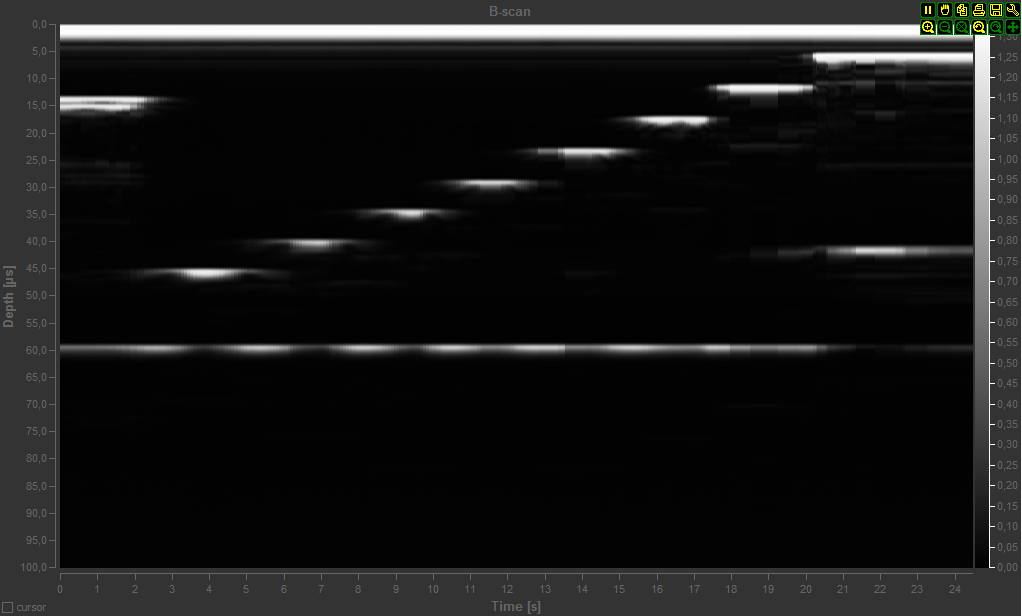
\includegraphics[scale=0.4]{BScan1.PNG}
  \caption{B-Scan des Acrylblocks in aufrechter Position.}
  \label{abb4}
\end{figure}

\FloatBarrier
\begin{figure}
  \centering
 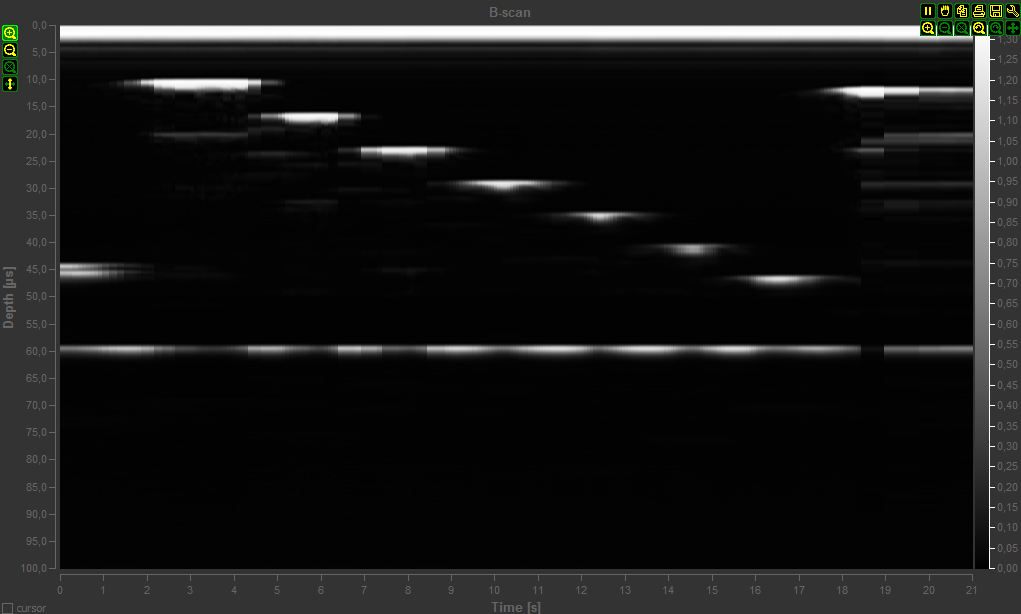
\includegraphics[scale=0.4]{BScan2.PNG}
 \caption{B-Scan des gedrehten Acrylblocks.}
 \label{abb5}
 \end{figure}
\FloatBarrier

\begin{table}
  \centering
  \caption{Messwerte und Ergebnisse der Untersuchung des Acrylblocks mittels B-Scans.}
  \label{tab4}
  \begin{tabular}{ c c c c c c }
    \toprule
    Störstelle & $\Delta t_d$ / $\si{\micro \second}$ & $d$ / $\si{\cm}$ & $\Delta t_s$ / $\si{\micro \second}$ & $s$ / $\si{\cm}$ & $l$ / $\si{\cm}$ \\
    \midrule
     1    &   13,8    &     1,88    &     45,9      &     6,27      &     $\SI{0,10(5)}{}$    \\
     2    &   15,3    &     2,09    &     44,4      &     6,06      &     $\SI{0,10(5)}{}$    \\
     3    &   45,9    &     6,27    &     10,9      &     1,49      &     $\SI{0,49(5)}{}$    \\
     4    &   40,3    &     5,50    &     17,0      &     2,32      &     $\SI{0,43(5)}{}$    \\
     5    &   34,8    &     4,75    &     23,2      &     3,17      &     $\SI{0,33(5)}{}$    \\
     6    &   29,3    &     4,00    &     29,5      &     4,03      &     $\SI{0,22(5)}{}$    \\
     7    &   23,6    &     3,22    &     35,2      &     4,80      &     $\SI{0,23(5)}{}$    \\
     8    &   17,9    &     2,44    &     41,3      &     5,64      &     $\SI{0,17(5)}{}$    \\
     9    &   11,8    &     1,61    &     46,8      &     6,39      &     $\SI{0,25(5)}{}$    \\
    10    &    6,3    &     0,86    &     -         &     -         &     -                   \\
    11    &   41,8    &     5,70    &     12,2      &     1,67      &     $\SI{0,88(5)}{}$    \\
    \bottomrule
    \end{tabular}
\end{table}
\FloatBarrier

\subsection{Untersuchung des Auflösevermögens}
Im folgenden Teil des Versuchs wird das Auflösevermögen zweier Schallköpfe untersucht, die unterschiedliche
Frequenzen besitzen, indem die zwei mit den Schallköpfen aufgenommenen A-Scans der Störstellen "1" und "2" miteinandern verglichen werden(siehe Abbildung \ref{abb3}).
Wird der einhüllenden FFT, die sich im Plot blau darstellt, die Amplitude des Schallkopfes zugeschaltet, so ist zu erkennen, dass kleine
Abstände, so wie der zwischen Störstelle "1" und "2" von der niedrigeren $\SI{1}{\mega \hertz}$-Sonde nicht gut aufgelöst werden können,
da der Schall durch die längere Laufzeit die Störstelle einfach "überläuft". Die $\SI{2}{\mega \hertz}$-Sonde hingegen liefert zwei Peaks,
die dich beieinander liegen, wovon auszugehen ist, dass dies die beiden Störstellen sind.
\FloatBarrier
\begin{figure}
    \centering
  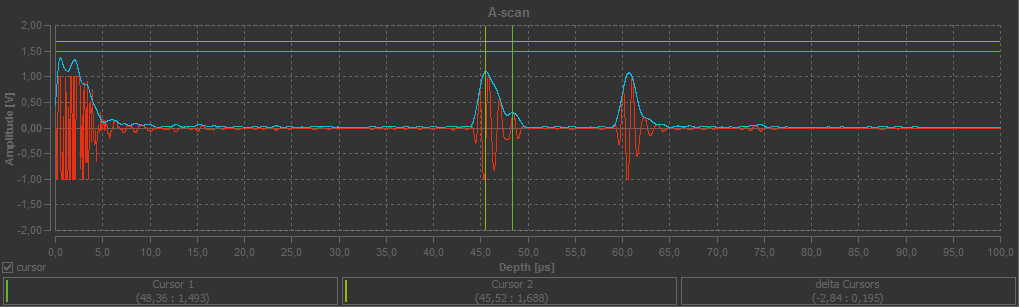
\includegraphics[scale=0.6]{1.2.1MHz.Frequenz.PNG}
  \caption{A-Scan der Störstellen "1" und "2" mit der $\SI{1}{\mega \hertz}$-Sonde.}
  \label{abb6}
\end{figure}
\FloatBarrier

\begin{figure}
  \centering
 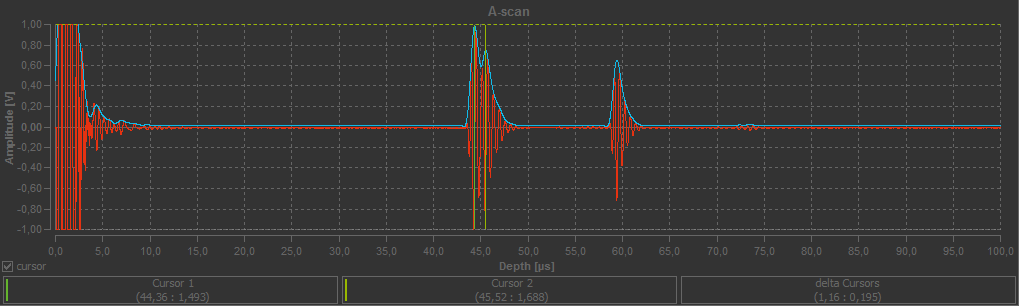
\includegraphics[scale=0.6]{1.2.2MHz.Frequenz.PNG}
 \caption{A-Scan der Störstellen "1" und "2" mit der $\SI{2}{\mega \hertz}$-Sonde.}
 \label{abb7}
\end{figure}
\FloatBarrier

\subsection{Untersuchung eines Herzmodells mit einem TM-Scan}
Um das Schlagvolumen des Herzmodells zu berechnen, wird die Laufzeit des Schalls von der Wasseroberfläche bis zum Boden und zurück vermessen, woraus
im folgenden die Wassertiefe und daraus das vom Wasser ausgefüllte Volumen berechnet werden können.
Die Laufzeit betrug $\SI{36,19}{\micro \second}$, was bei einer Schallgeschwindigkeit in Wasser von $\SI{1485}{\metre \per \second}$ \cite{Q2} eine
Wassertiefe von $h$ = $\SI{2,69}{\cm}$ , die mittels Formel \ref{eq1} berechnet wurde. Das enddiastolische Volumen $V_d$ und der zugehörige
Fehler $\Delta V_d$, der dadurch entsteht, dass die Messung des Zylinderdurchmessers ($d$ = $\SI{4,57(5)}{\cm}$) mit der Schieblehre fehlerbehaftet ist, berechnen sich
mittels folgender Gleichungen:
\FloatBarrier
\begin{align*}
  V_d &= \pi \cdot (\frac{d}{2})^2 \cdot h &= \SI{44,08}{\cm \squared}    \\
  \Delta V_d &=  h \pi~\frac{d}{2} \cdot \Delta d &= \pm \SI{0,97}{\cm \squared}    \\
\end{align*}
\FloatBarrier
Das endsystolische Volumen mit zugehörigem Fehler errechnet sich analog mit einer Schalllaufzeit von $\SI{6,45}{\micro \second}$ zu
\begin{align*}
  V_s &= \SI{3,44(17)}{\cm \squared} ~ .
\end{align*}
\FloatBarrier
Das Schlagvolumen berechnet sich aus der Differenz zwsichen endsystolischem und enddiastolischem Volumen zu $V$ = $\SI{40,64(141)}{\cm \squared}$.
Mit einem Time-Motion Scan wird dann das rhythmische Pumpen des Herzmodells aufgenommen, was in Abbildung \ref{abb8} zu sehen ist.
Aus dem mittleren Abstand der Maxima lässt sich die Herzfrequenz ermitteln: Im Time-Motion-Scan sind innerhalb von $\SI{20}{\second}$ sieben Maxima registriert,
was einer Herzfrequenz von 21 Schlägen pro Minute entspricht.
Das Herzvolumen kann ebenfalls aus der Kurve ermittelt werden, indem die Laufzeitdifferenz zwischen Maximum und Minimum der dargestellten Kurve
ermittelt wird. Diese beträgt für die erste Amplitude $\SI{37,5}{\micro \second}$. Dies entspricht der Höhe des gepumpten Wassers im Zylinder.
Somit ergibt sich ein Schlagvolumen von $V$ = $\SI{45,67(100)}{\cm \squared}$. Das Herzvolumen berechnet sich aus der Summe des Schalgvolumens
und dem endsystolischen Volumen und beträgt folglich:
\begin{align*}
  V_{\symup{gesamt}} &= \SI{49,11(117)}{\cm \squared} ~.
\end{align*}
\FloatBarrier
\begin{figure}
  \centering
 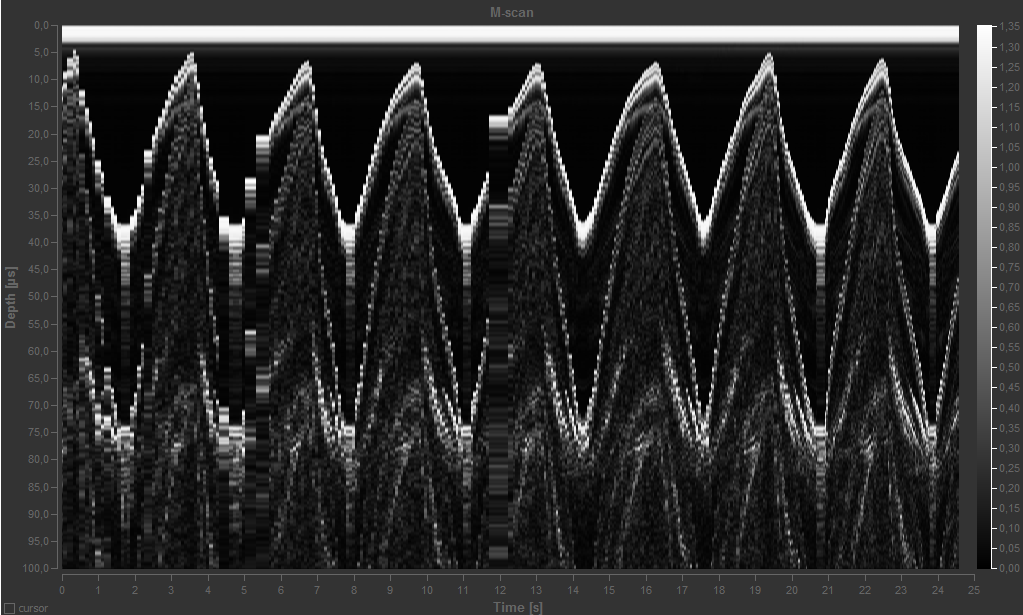
\includegraphics[scale=0.6]{Herz.PNG}
 \caption{TM-Scan des pumpenden Herzmodells.}
 \label{abb8}
\end{figure}
\FloatBarrier

\section{Diskussion}
\FloatBarrier
In Tabelle \ref{tab5} sind die Durchmesser der Störstellen $l_{\symup{A,B}}$, die mittels A- und B-Scan
ermittelt wurden, mit prozentualer Abweichung von den, mit der Schieblehre, gemessenen Durchmessern $l_{\symup{g}}$ dargestellt.
\FloatBarrier
\begin{table}
  \centering
  \caption{Ergebnisse des Versuchs im Vergleich.}
  \label{tab4}
  \begin{tabular}{ c c c c c c }
    \toprule
    Störstelle & $l_{\symup{g}}$ / $\si{\cm}$ & $l_{\symup{A}}$ / $\si{\cm}$ & $\Delta \symup{A}$ / $\si{\percent}$ &  $l_{\symup{B}}$ / $\si{\cm}$ & $\Delta \symup{B}$ / $\si{\percent}$\\
    \midrule
     1    &   $\SI{0,15(5)}{}$    &   -                      &  -       &   $\SI{0,10(5)}{}$    &   33,3       \\
     2    &   $\SI{0,15(5)}{}$    &   -                      &  -       &   $\SI{0,10(5)}{}$    &   33,3       \\
     3    &   $\SI{0,60(5)}{}$    &   $\SI{0,89(5)}{}$       &   48,3   &   $\SI{0,49(5)}{}$    &   18,3       \\
     4    &   $\SI{0,50(5)}{}$    &   $\SI{0,77(5)}{}$       &   54,0   &   $\SI{0,43(5)}{}$    &   14,0       \\
     5    &   $\SI{0,41(5)}{}$    &   $\SI{0,68(5)}{}$       &   65,9   &   $\SI{0,33(5)}{}$    &   19,5       \\
     6    &   $\SI{0,30(5)}{}$    &   $\SI{0,60(5)}{}$       &  100,0   &   $\SI{0,22(5)}{}$    &   26,7       \\
     7    &   $\SI{0,30(5)}{}$    &   $\SI{0,54(5)}{}$       &   80,0   &   $\SI{0,23(5)}{}$    &   23,3       \\
     8    &   $\SI{0,30(5)}{}$    &   $\SI{0,57(5)}{}$       &   90,0   &   $\SI{0,17(5)}{}$    &   43,3       \\
     9    &   $\SI{0,30(5)}{}$    &   $\SI{0,57(5)}{}$       &   90,0   &   $\SI{0,25(5)}{}$    &   16,7       \\
    10    &   $\SI{0,30(5)}{}$    &   -                      &  -       &   -                   &   -          \\
    11    &   $\SI{1,00(5)}{}$    &   $\SI{1,00(5)}{}$       &   0      &   $\SI{0,88(5)}{}$    &   12,0       \\
    \bottomrule
    \end{tabular}
\end{table}
\FloatBarrier
Bei der Betrachtung des Vergleichs der Durchmesser der Störstellen fällt auf, dass die mittels B-Scan ermittelten Störstellen deutlich kleinere
Abweichungen zeigen. Eine Erklärung dafür ist, dass die B-Scans mit einer $\SI{2}{\mega \hertz}$-Sonde erstellt wurden. Im Gegensatz dazu wurde
zur Erstellung der A-Scans lediglich eine $\SI{1}{\mega \hertz}$-Sonde verwendet. Die so vermutete bessere Auflösung durch Sonden, die eine höhere
Schallfrequenz aussenden, deckt sich mit den Ergebnissen aus dem Versuchsteil, in dem die beiden kleinsten Störstellen untersucht werden.
Der Durchmesser der Störstelle mit der Nummerierungsnummer 10 kann wegen der Größe der Störstelle 11 nicht ermittelt werden. Der Durchmesser
von $\SI{1}{cm}$ ist hierbei eine zu dicke luftgefüllte Barriere, durch die das Ultraschallsignal nicht hindurch dringen kann.
Bei der Untersuchung der Auflösungsqualität ist zu erkennen, dass eine Sonde mit höhrere Schallfrequenz besser kleine Ungenauigkeiten darstellt, als
eine Sonde mit niedrigerer Frequenz. Dies liegt daran, dass bei niedrigeren Frequenzen im A-Scan die Amplitudenbreite breiter als die zu detektierende
Fehlstelle wird und diese somit nicht erfasst wird. Eine höhere Auflösung wäre durch noch größere Frequenzen des Schallkopfes möglich.
Zur Bestimmung des Herzvolumens mittels des TM-Scans ist zu sagen, dass die Amplitude des Herzschlags nicht mit Hilfe des Cursors, sondern lediglich
nachträglich an der nicht ausreichend beschrifteten Skala abgelesen wurde. Hier ist also davon auszugehen, dass dies die Große Abweichung von
$\SI{11}{\percent}$zu dem, zuvor direkt ermittelten, Herzvolumen mittels des A-Scans erklärt.

\nocite{*}
\printbibliography
